\clearpage

\def\testeimplies{\mathrel{\ensurestackMath{\stackon[1pt]{\implies}{\scriptstyle t_0 \equiv 0}}}}
\def\testeimpliess{\mathrel{\ensurestackMath{\stackon[1pt]{\implies}{\scriptstyle v_z(t_1^-) < 0}}}}
%//==============================--@--==============================//%
%\vspace{-1em}
\subsection{P1 | Simulação do movimento da bola (somente na vertical)}
\label{subsec:P1}

De modo a caracterizar as condições \underline{base} de partida que fomentam o estudo dos efeitos do coeficiente de restituição $\alpha$, e da velocidade inicial $v_z(t_0^+)$, apresentam-se abaixo, na \hyperref[fig:P1-SistemaCompleto]{Fig. 2}, a evolução temporal da posição da bola saltitante e da sua velocidade vertical para $z(t_0) := z_0 = 10$ m, $v_{z}(t_0^+) := v_{z_0} = 0$ ms$^{-1}$ e $\alpha = 0.8$. 

\begin{wrapfigure}[14]{l}{0.575\textwidth}
    \centering
    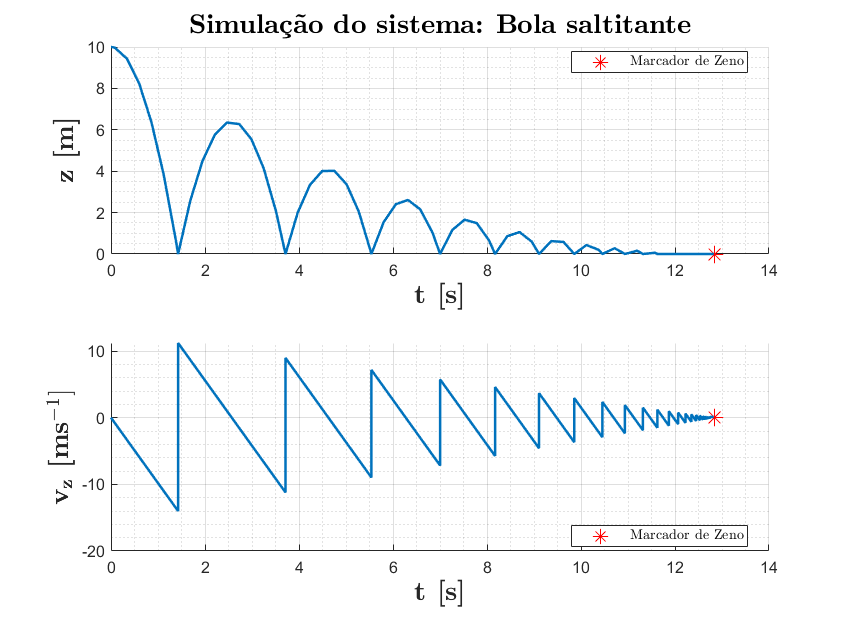
\includegraphics[width=0.575\textwidth]{img/P1/P1-SistemaCompleto.png}
    \caption{Simulação do sistema para as condições iniciais supramencionadas e $\alpha = 0.8$ ($t_0 \equiv 0$).}
    \label{fig:P1-SistemaCompleto}
\end{wrapfigure}

\vphantom{123}

\noindent\textbf{\textit{$\rightarrow$ Observações}}
\vspace{-0.5em}
\begin{itemize}
    \item[$\blacktriangle$] Verifica-se a descontinuida- de da velocidade no instan- te de embate da bola com a superfície (\textit{jump})\protect\footnotemark[3].
    
    \item[$\blacktriangle$] Afunilamento sucessivo ex- pectável da velocidade com base nas perdas energéticas.
    
    \item[$\blacktriangle$] A bola saltitante é incapaz de atingir a posição vertical inicial graças à dissipação energética imposta pelo fator $\alpha = 0.8$.
\end{itemize}

\footnotetext[3]{Denota-se a velocidade logo antes e após o choque com os $-$ e $+$ sobrescritos, respetivamente.}

\vspace{1em}
\noindent A posição vertical da massa pontual em períodos de \textit{flow} é regida pela equação:
\vspace{-0.5em}
$$
    z(t + t_{n-1}) = z(t_{n-1}) + v_{z}(t_{n-1}^+) \cdot t - \frac{1}{2}g \cdot t^2\qquad n = 1, 2, \dots
$$

\vspace{-0.5em}
\noindent em que $z(t_{n-1})$ é a altura inicial do período de \textit{flow}\footnotemark[4] $n$, e $v_{z}(t_{n-1}^+)$ a velocidade inicial desse mesmo período (para $n \ge 2$, será a velocidade após o \textit{jump} \hyperref[sec:intro]{definido acima}).

\footnotetext[4]{A altura inicial é nula para todos os períodos de \textit{flow} subsequentes ao 1\textordmasculine{} ($n \ge 2: z(t_{n-1}) \equiv 0$). Para o primeiro período ($n=1$), são assumidas as condições iniciais impostas: $z_0$ e $v_{z_0}$.}

Relembrando a \underline{Lei de Conservação d'Energia}: $\Delta E = \Delta T + \Delta U = 0$ (dado que não são aplicadas forças externas ao sistemas ao longo de cada período de \textit{flow}), trivialmente se obtém $v_{z}$ imediatamente antes do primeiro choque:
\vspace{-0.5em}
$$
    \Delta E = 0 \iff mg z_0 + \frac{1}{2}m (v_{z_0})^2 = \frac{1}{2}m [v_{z}(t_{1}^-)]^2 \:\testeimpliess\: v_z(t_{1}^-) = -\sqrt{2 g z_0 + (v_{z_0})^2}
$$

\vspace{-0.5em}
\noindent Para condições iniciais arbitrárias, o tempo acumulado após $N$ choques é dado por:

\vspace{-0.5em}
$$
    T_N = t_1 + t_2 + t_3 + \dots = \frac{v_{z_0}}{g} +  \frac{\sqrt{2 g z_0 + (v_{z_0})^2}}{g} \left(1 + 2 \sum\limits_{n=1}^{N-1} \alpha^n \right)
$$
em que $t_n$ representa a duração\footnotemark[5] do $n$-ésimo período de \textit{flow}, para $n \in \mathbb{N}$.

A série geométrica com razão $\alpha$, converge para valores do coeficiente $\alpha \in [0,\,1[$. Define-se finalmente o tempo em que ocorre o \hyperref[def:zeno]{fenómeno de Zeno}\footnotemark[9]\footnotemark[10]:
\vspace{-0.5em}
$$
    \therefore T_{Zeno} := \lim\limits_{N \to +\infty} T_N = \frac{1}{g} \left(v_{z_0} + \sqrt{2 g z_0 + (v_{z_0})^2} \left(\frac{1+\alpha}{1-\alpha}\right)\right),\quad \alpha \in [0,\,1[
$$

\vspace{-0.5em}
\noindent \textbf{Nota} $\pmb{\rightarrow}$ Conceptualmente, $T_{Zeno}$ pode ser visto como o tempo \underline{teórico} necessário até que ``\textit{(...) the ball settles down to the ground with zero velocity (...)}''\cite{mathworks-bouncingball}.

\footnotetext[5]{Note-se que $t_n$ é a solução positiva da equação quadrática $z(t+t_{n-1}) = 0$, para $n = 1, 2, \dots$ ($t_0 \equiv 0$).}
%//==============================--C--==============================//%
\clearpage

\noindent $\pmb{\rightarrow}$ \textbf{\textit{Condições iniciais e fenómeno de Zeno}}

\noindent Para as condições iniciais \hyperref[fig:P1-SistemaCompleto]{expostas acima} e $\alpha = 0.8$, obtém-se $T_{Zeno} = 12.8506\text{ s}$. Este fenómeno é capturado em ambiente de simulação através da deteção (\textit{default}) de \textit{consecutive zero crossing events} em intervalos de tempo ínfimos:

\begin{warning}
    \footnotesize\color{red}\texttt{An error occurred while running the simulation (...): Simulink will stop the simulation of model 'P1simulink' because the 1 zero crossing signal(s) identified below caused 1000 consecutive zero crossing events in time interval between 12.850588106411884 and 12.850588107006466.}
\end{warning}

\vspace{-0.5em}
\noindent Na \hyperref[fig:P1-SistemaCompleto]{Fig. 2 acima}, este comportamento é delimitado pelo "marcador de Zeno" ({\color{red} $\star$}).

De modo a garantir a generalidade da discussão, explora-se a (expectável) relação íntima entre o fator de atenuação e da velocidade inicial com o valor de $T_{Zeno}$. 

%\setcounter{footnote}{0}
%\renewcommand*{\thefootnote}{\fnsymbol{footnote}}
\vspace{-0.75em}
\begin{figure}[H] 
    \begin{subfigure}[b]{0.33\linewidth}
        \centering
        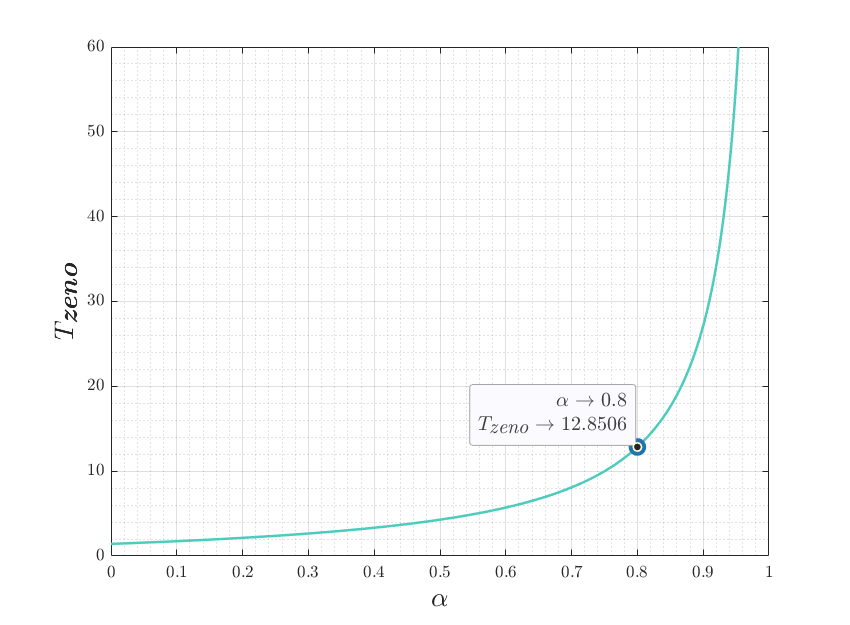
\includegraphics[width=1\linewidth]{img/P1/P1-coefTimpacto.png}
        \caption{$T_{Zeno}$: variação de $\alpha$ para $z_0 = 10$ m e $v_{z_0} = 0$ ms$^{-1}$} 
        \label{fig:coefTimpacto} 
    \end{subfigure}%% 
    \begin{subfigure}[b]{0.33\linewidth}
        \centering
        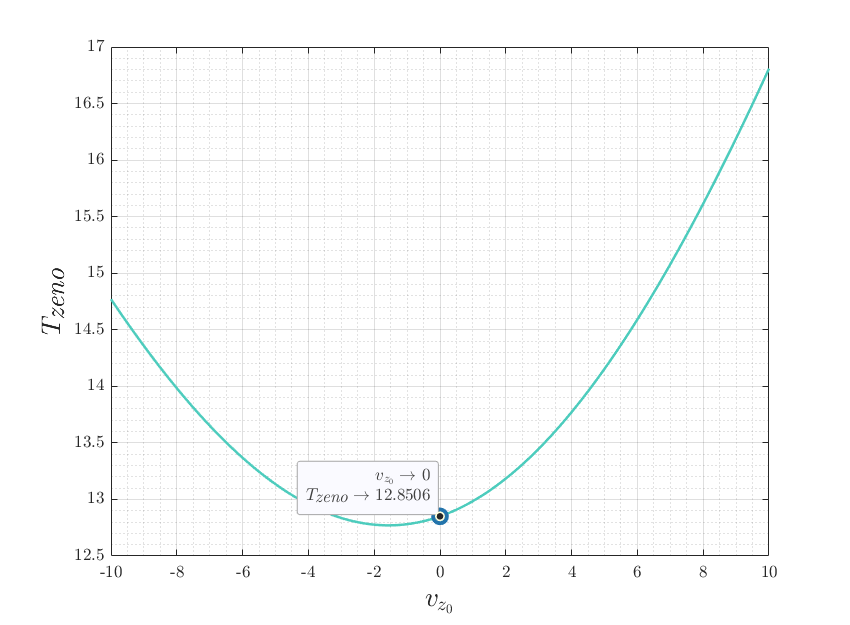
\includegraphics[width=1\linewidth]{img/P1/P1-veloTinf.png} 
        \caption{$T_{Zeno}$: variação de $v_{z_0}$ para $z_0 = 10$ m e $\alpha = 0.8$} 
        \label{fig:veloTinf} 
    \end{subfigure}
    \begin{subfigure}[b]{0.33\linewidth}
        \centering
        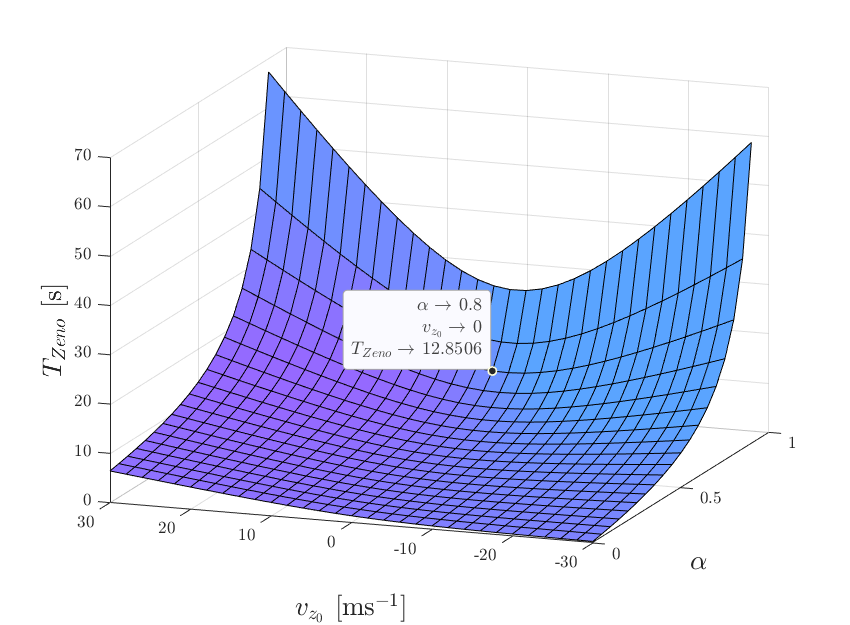
\includegraphics[width=1\linewidth]{img/P1/P1-3dplot.png} 
        \caption{$T_{Zeno}$: variação de $v_{z_0}$ e de $\alpha$, para $z_0 = 10$ m} 
        \label{fig:3dplot} 
    \end{subfigure} 
    \caption{Efeito da variação de $\alpha$ e $v_{z_0}$ no valor de $T_{Zeno}$. Note-se que, naturalmente, uma diminuição de $\alpha$ traduz-se numa diminuição de $T_{Zeno}$, e vice-versa\protect\footnotemark[6] (\textit{vide} \hyperref[fig:phase-portrait-limites]{Fig. 6}) $\rightarrow$ comportamento de acordo com a dinâmica energética do sistema imposta por este parâmetro. Curiosamente, verifica-se que ao alterar a energia inicial do sistema, impondo uma velocidade inicial (para um $\alpha \in\, ]0,\, 1[$), despoleta uma evolução de $T_{Zeno}$---não óbvia---visível na \hyperref[fig:veloTinf]{curva (b)}. Verifica-se que o valor de $v_{z_0}$ que minimiza $T_{Zeno}$, para um determinado $\alpha$ fixo (e $z_0 \in \mathbb{R}_{>0}$), é sempre inferior a $0$\protect\renewcommand*{\thefootnote}{\fnsymbol{footnote}}\protect\footnotemark[2] (\hyperref[fig:Derivada]{Fig. 4 (a)}).}
\end{figure}

\renewcommand*{\thefootnote}{\arabic{footnote}}
\footnotetext[6]{Do outro lado do espectro, um $\alpha \to 1$ implica um aumento avassalador de $T_{Zeno}$ ($\to +\infty$), como aparente na \hyperref[fig:matrixcoef]{Fig. 4 (c)} e nos \hyperref[fig:phase-portrait]{retratos de fase subsequentes}.}

\footnotetext[7]{O $v_{z_0}$ minimizante de $T_{Zeno}$ diminui o intervalo de tempo até ao 1\textordmasculine{} choque, não aumentando substancialmente os períodos de \textit{flow} subsequentes.}

\renewcommand*{\thefootnote}{\fnsymbol{footnote}}
\footnotetext[2]{ 
$
    \left.\dfrac{\partial T_{Zeno}}{\partial v_{z_0}}\right\vert_{\alpha} = 
    \dfrac{1}{g}\left(\cfrac{v_{z_0}}{\sqrt{2 g z_0 + (v_{z_0})^2}}\left(\dfrac{1+\alpha}{1-\alpha}\right)+1\right) =
    0
    \implies
    v_{z_0}\biggr\rvert_{\alpha} = -\sqrt{\dfrac{g z_0 \left( 1-\alpha \right)^2}{2\alpha}}
$ \hfill\raisebox{-0.8 em}{\ensuremath{\Box}}
}

%\noindent experiência %sim adoro-te :3
\vspace{-1em}
\noindent Como lembra a Análise Matemática, o valor de $v_{z_0}$ que minimiza $T_{Zeno}$ (mínimo local) para um dado $\alpha$, é deduzido através da 1\textordfeminine{} derivada parcial em ordem a $v_{z_0}$\footnotemark[2]$\mkern-1mu^{,}$\renewcommand*{\thefootnote}{\arabic{footnote}}\footnotemark[7].

\renewcommand*{\thefootnote}{\fnsymbol{footnote}}

\vspace{-0.75em}
\begin{figure}[ht] 
     \begin{subfigure}[b]{0.33\linewidth}
        \centering
        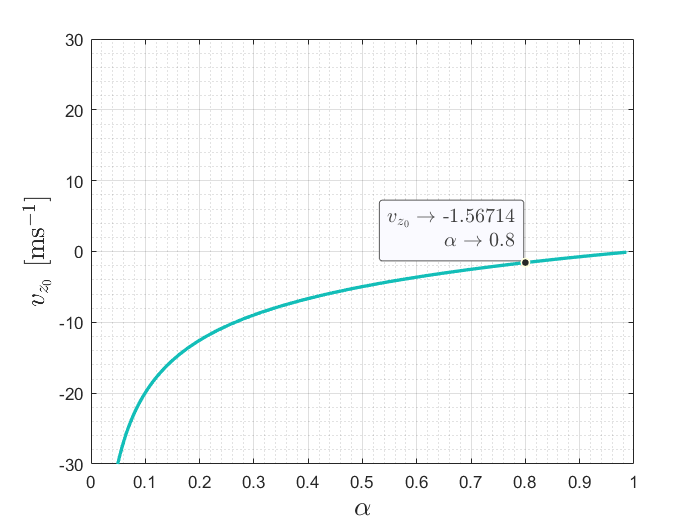
\includegraphics[width=1\linewidth]{img/P1/P1-DerivadaShenanigan.png} 
        \caption{$(\partial T_{Zeno}/\partial v_{z_0})|_{\alpha} = 0 $\protect\footnotemark[2]\\ \vphantom{}} 
        \label{fig:Derivada} 
    \end{subfigure}%%
    \begin{subfigure}[b]{0.33\linewidth}
        \centering
        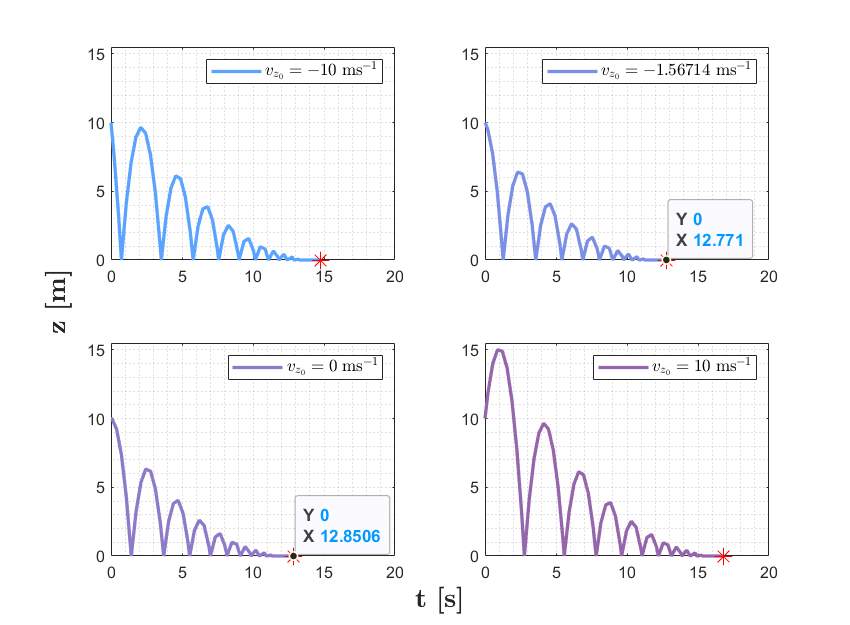
\includegraphics[width=1\linewidth]{img/P1/P1-velomatrix.png} 
        \caption{Posição vertical da bola para $v_{z_0}$ variável ($\alpha = 0.8$).} 
        \label{fig:matrixvelo} 
    \end{subfigure}%%
    \begin{subfigure}[b]{0.33\linewidth}
        \centering
        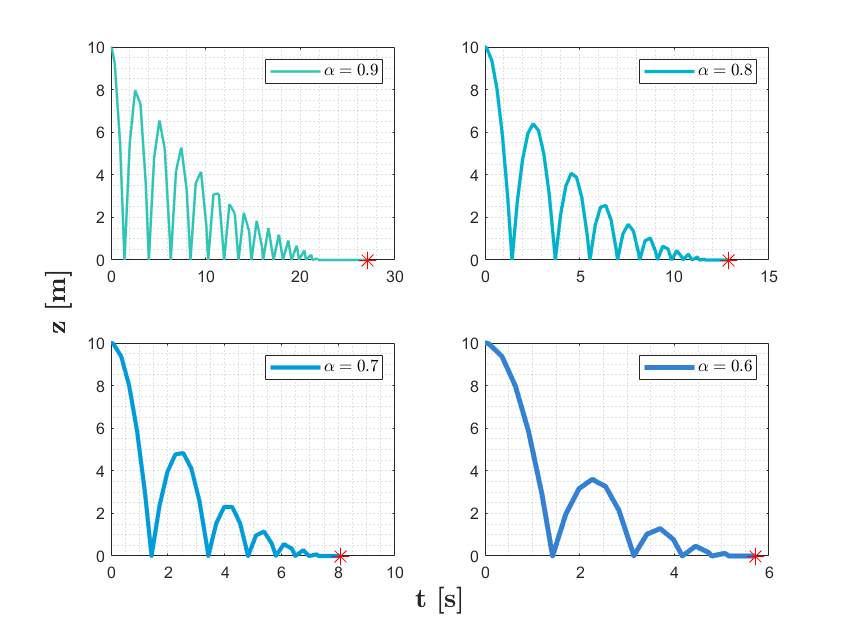
\includegraphics[width=1\linewidth]{img/P1/P1-coefmatrix.png}
        \caption{Posição vertical da bola para $\alpha$ variável ($v_{z_0} = 0$ ms$^{-1}$).} 
        \label{fig:matrixcoef} 
    \end{subfigure}%%
    \caption{Curva de nível da derivada parcial de $T_{Zeno}$ em ordem a $v_{z_0}$\protect\footnotemark[2] e visualização temporal da posição vertical da massa puntiforme relativamente a alguns exemplos que espelham o efeito da variação da velocidade inicial e do fator de atenuação (para um $z_0 = 10$ m).}
\end{figure}

%\setcounter{footnote}{4}
\renewcommand*{\thefootnote}{\arabic{footnote}}

%//==============================--A--==============================//%
\clearpage
\noindent $\pmb{\rightarrow}$ \textbf{\textit{Retratos de fase}}

\noindent O efeito do coeficiente de restituição $\alpha$ e de $v_{z_0}$ são apresentados condensadamente através da visualização dos retratos de fase do sistema. Note-se: para valores de $\alpha\in [0,\, 1[$ ocorre uma diminuição (expectável) da velocidade vertical após cada impacto e consequentemente da altura máxima\footnotemark[8] atingida pela massa pontual no período de \textit{flow} que sucede o embate com a superfície horizontal. Este fenómeno é cada vez mais acentuado para valores de $\alpha$ sucessivamente mais próximos de $0$ (\textit{vide} \hyperref[fig:phase-portrait-limites]{Fig. 6}).

\footnotetext[8]{Denominaremos por $z_\textit{máx}$ este valor daqui em diante.}

\vspace{-0.65em}
\begin{figure}[H]
    \centering
    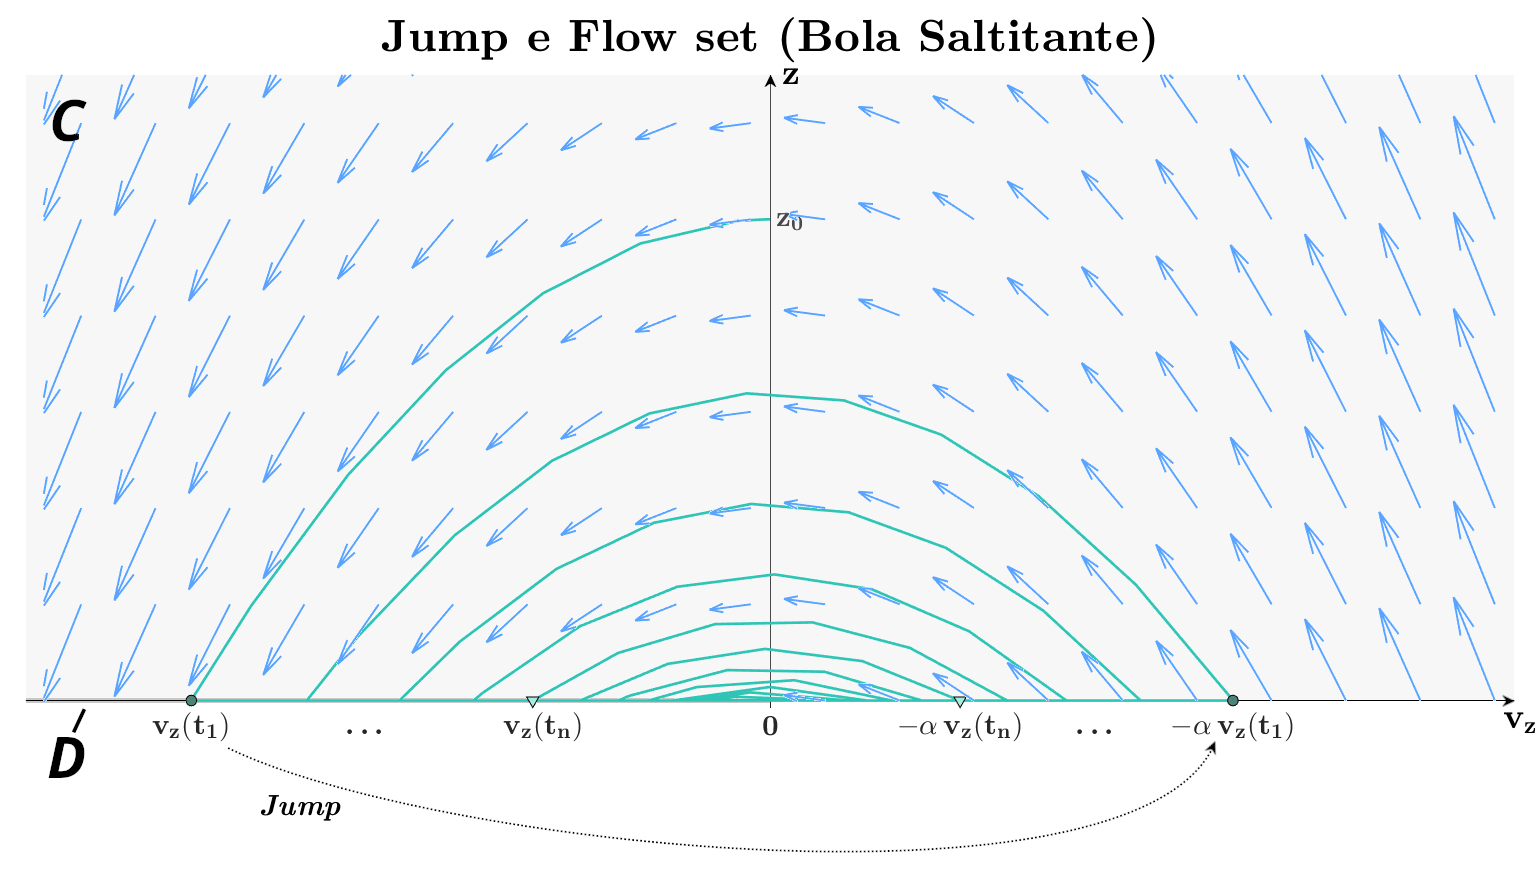
\includegraphics[width = 0.9\linewidth]{img/P1/P1-PhasePortrait.png}
    \caption{Retrato de fase do sistema para $z_0 = 10$ m, $v_{z_0} = 0$ ms$^{-1}$ e $\alpha = 0.8$. (Exemplo que traduz a resposta para valores de $\alpha \in\, ]0,\, 1[$ $\rightarrow$ \textbf{colisões elásticas}\protect\footnotemark[9] $\rightarrow$ perdas energéticas com o embate na superfície; salienta-se a diminuição dos intervalos entre colisões---resposta naturalmente esperada para o caso exposto, cada vez mais acentuada para valores de $\alpha$ cada vez mais pequenos).}
    \label{fig:phase-portrait}
\end{figure}

\footnotetext[9]{``\textit{It is easily shown that if the impacts are not perfectly elastic, the ball displays Zeno behavior}''\cite{Or2011-db}.}

\vspace{-1.25em}
\begin{figure}[ht] 
    \begin{subfigure}[b]{0.5\linewidth}
        \centering
        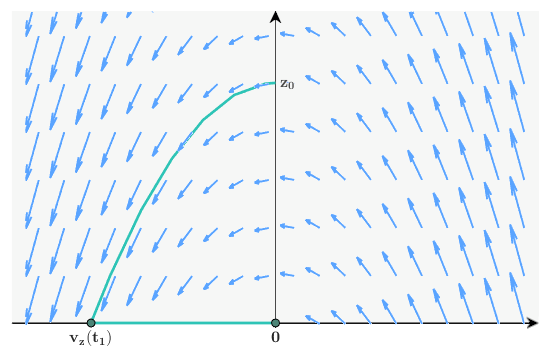
\includegraphics[width=1\linewidth]{img/P1/P1-PhasePortrait-alpha=0.png}
        \caption{Retrato de fase para $z_0 = 10$ m, $v_{z_0} = 0$ ms$^{-1}$ e\\ $\pmb{\underline{\alpha = 0}}$.} 
        \label{fig:phase-portrait-alpha0} 
    \end{subfigure}%% 
    \begin{subfigure}[b]{0.5\linewidth}
        \centering
        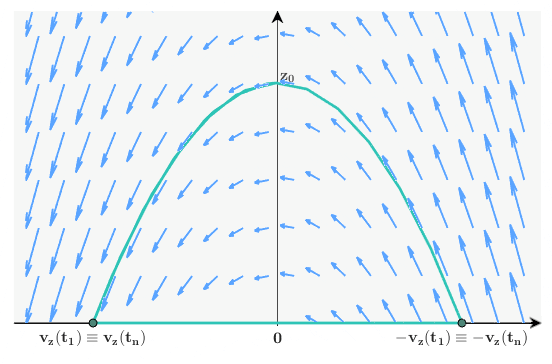
\includegraphics[width=1\linewidth]{img/P1/P1-PhasePortrait-alpha=1.png} 
        \caption{Retrato de fase para $z_0 = 10$ m, $v_{z_0} = 0$ ms$^{-1}$ e\\ $\pmb{\underline{\alpha = 1}}$.} 
        \label{fig:phase-portrait-alpha1} 
    \end{subfigure} 
    \caption{Comportamento do sistema da bola saltitante para os casos limites em que o coeficiente de restituição $\alpha$ toma os valores: $\pmb{0}$ (\textbf{colisão inelástica} $\rightarrow$ perda máxima de energia $\rightarrow \pmb{T_{Zeno} = t_1}$) e $\pmb{1}$ (\textbf{colisão perfeitamente elástica} $\rightarrow$ conservação total da energia cinética $\rightarrow \pmb{T_{Zeno} \to +\infty}$).}
    \label{fig:phase-portrait-limites}
\end{figure}

\vspace{-1em}
\noindent Acresce-se ainda o reparo: para $\alpha = 0$ existe somente um período de \textit{flow}\footnotemark[10] dado que toda a energia cinética é perdida com o choque e a massa pontual permanece, deste modo, pegada à superfície; para $\alpha = 1$ o comportamento repete-se \textit{ad aeternum}\footnotemark[10].

\footnotetext[10]{Para os casos limites $\alpha \in \{0, 1\}$, não se verifica o efeito de Zeno (\textit{vide} \hyperref[def:zeno]{secção introdutória}).}
%//==============================--@--==============================//%